\chapter{Phonon Anomalies in LSCO+O}\label{ch:anomaly}

\section{Origin of the phonon anomaly}
Phonon anomalies in materials can, in general, happen for a number of reasons. The Cu-O bond-stretching phonon anomaly in LSCO does not seem to be caused by any of the conventional phenomena, and a relationship to novel charge modes has been proposed. One such charge mode is fluctuations of stripe order. The appeal of this interpretation is the near impossibility of measuring dynamic charge stripes directly. The phonon anomaly could thus provide an indirect way of investigating the elusive properties of dynamic charge stripes. Given the hypothesis that the phonon anomaly and dynamic charge stripes are related, what are then the possible mechanisms of the coupling? A couple of scenarios are given in Figure \ref{fig:anomaly_2d} and \ref{fig:anomaly_1d}.

The charge oscilation was introduced by \citeauthor{Kaneshita2002}\cite{Kaneshita2002} in a theoretical study of stripes coupling to the phonon. The Kohn anomaly picture was introduced in context of LBCO by \citeauthor{Reznik2006}\cite{Reznik2006} as an intuitive way to explain the connection between the phonon and stripe wavevectors. The 2D picture in Figure \ref{fig:anomaly_2d} has only been mentioned (to my knowledge) by \citeauthor{Reznik2010} in his two reviews on the phonon anomaly\cite{Reznik2010, Reznik2012}. Note, it appears that the Kohn anomaly picture has been ruled out by ARPES measurements by \citeauthor{Park2014}\cite{Park2014}

\begin{figure}
    \centering
    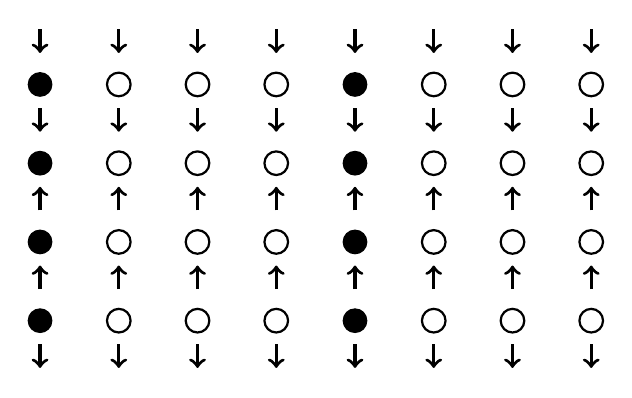
\begin{tikzpicture}
    % charge stripe
    \foreach \y in {0,1,2,3} {
        \foreach \x in {0,4} {
            \filldraw (\x+0,\y) circle [radius=0.15];
            % afm
            \draw [thick] (\x+1,\y) circle [radius=0.15];
            \draw [thick] (\x+2,\y) circle [radius=0.15];
            \draw [thick] (\x+3,\y) circle [radius=0.15];
        }
    }
    
    \foreach \x in {0,1,2,3,4,5,6,7} {
        \draw [very thick, <-] (\x,-0.6) -- (\x,-0.3);
        \draw [very thick, ->] (\x,-0.6+1) -- (\x,-0.3+1);
        \draw [very thick, ->] (\x,-0.6+2) -- (\x,-0.3+2);
        \draw [very thick, <-] (\x,-0.6+3) -- (\x,-0.3+3);
        \draw [very thick, <-] (\x,-0.6+4) -- (\x,-0.3+4);
    }
\end{tikzpicture}
    \caption[2D phonon anomaly sketch]{Possible 2D real-space scenarios of a coupling between the Cu-O bond-stretching phonon at $q=(0.25,0.25,0)$ and stripe order. Here, the phonon wavector is perpendicular to the stripe direction (parallel to the stripe propagation vector). Small arrows represent displacement of oxygen atoms. Charge oscillations are phason modes of the stripes and the black bars represent charge domain walls. The Lower figure refers to a situation where static charge order lowers the energy of the phonon (intuitively through the change of spring constant). open circles represent hole-poor anti-ferromagnetic Cu atoms and filled circles represent hole-doped ($\frac{1}{2}$ hole per site) Cu atoms.}
    \label{fig:anomaly_1d}
\end{figure}

\begin{figure}
    \centering
    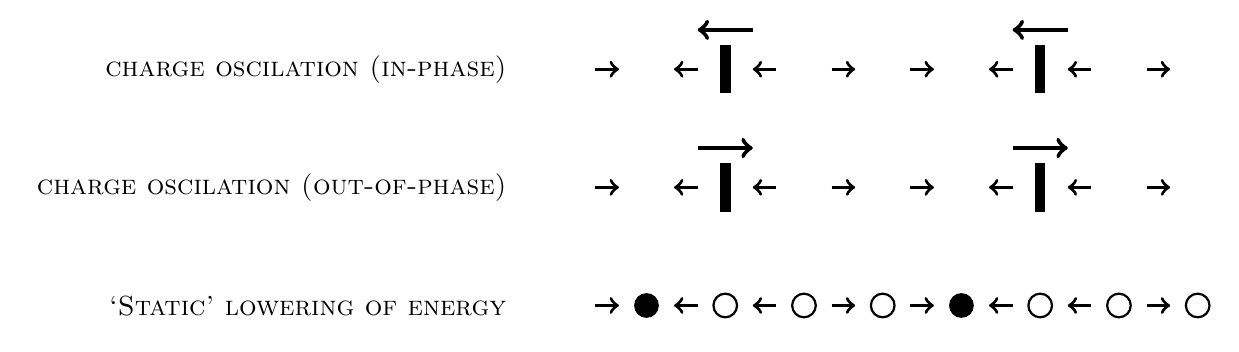
\begin{tikzpicture}
    % domain wall movement
    \foreach \y in {1.5,3} {
        \foreach \x in {0,4} {
            \draw [->, very thick] (\x,\y) -- (\x+0.3,\y);
            \draw [<-, very thick] (\x+1,\y) -- (\x+1.3,\y);
            \draw [<-, very thick] (\x+2,\y) -- (\x+2.3,\y);
            \draw [->, very thick] (\x+3,\y) -- (\x+3.3,\y);
        }
    }
    % domain walls
    \filldraw (1.59, 1.2) rectangle (1.71, 1.8);
    \draw [->, ultra thick] (1.3,2.0) -- (2.0,2.0);
    \filldraw (1.59+4, 1.2) rectangle (1.71+4, 1.8);
    \draw [->, ultra thick] (1.3+4,2.0) -- (2.0+4,2.0);
    \filldraw (1.59+4, 1.2+1.5) rectangle (1.71+4, 1.8+1.5);
    \draw [<-, ultra thick] (1.3,2.0+1.5) -- (2.0,2.0+1.5);
    \filldraw (1.59, 1.2+1.5) rectangle (1.71, 1.8+1.5);
    \draw [<-, ultra thick] (1.3+4,2.0+1.5) -- (2.0+4,2.0+1.5);
    
    % charge stripe
    \foreach \x in {0,4} {
        \draw [->, very thick] (\x,0) -- (\x+0.3,0);
        \draw [<-, very thick] (\x+1,0) -- (\x+1.3,0);
        \draw [<-, very thick] (\x+2,0) -- (\x+2.3,0);
        \draw [->, very thick] (\x+3,0) -- (\x+3.3,0);
        % charge
        \filldraw (\x+0.65,0) circle [radius=0.15];
        % afm
        \draw [thick] (\x+1.65,0) circle [radius=0.15];
        \draw [thick] (\x+2.65,0) circle [radius=0.15];
        \draw [thick] (\x+3.65,0) circle [radius=0.15];
    }
    
    \node [left] at (-1,0) {\textsc{`Static' lowering of energy}};
    \node [left] at (-1,1.5) {\textsc{charge oscilation (out-of-phase)}};
    \node [left] at (-1,3.0) {\textsc{charge oscilation (in-phase)}};
\end{tikzpicture}
    \caption[1D phonon anomaly sketch]{Possible 1D (Kohn Anomaly) scenario of the phonon anomaly. In this case the phonon wavevector resonates with the charge component parallel to the the stripes (perpendicular to the stripe propagation vector).}
    \label{fig:anomaly_2d}
\end{figure}

\begin{figure}
    \centering
    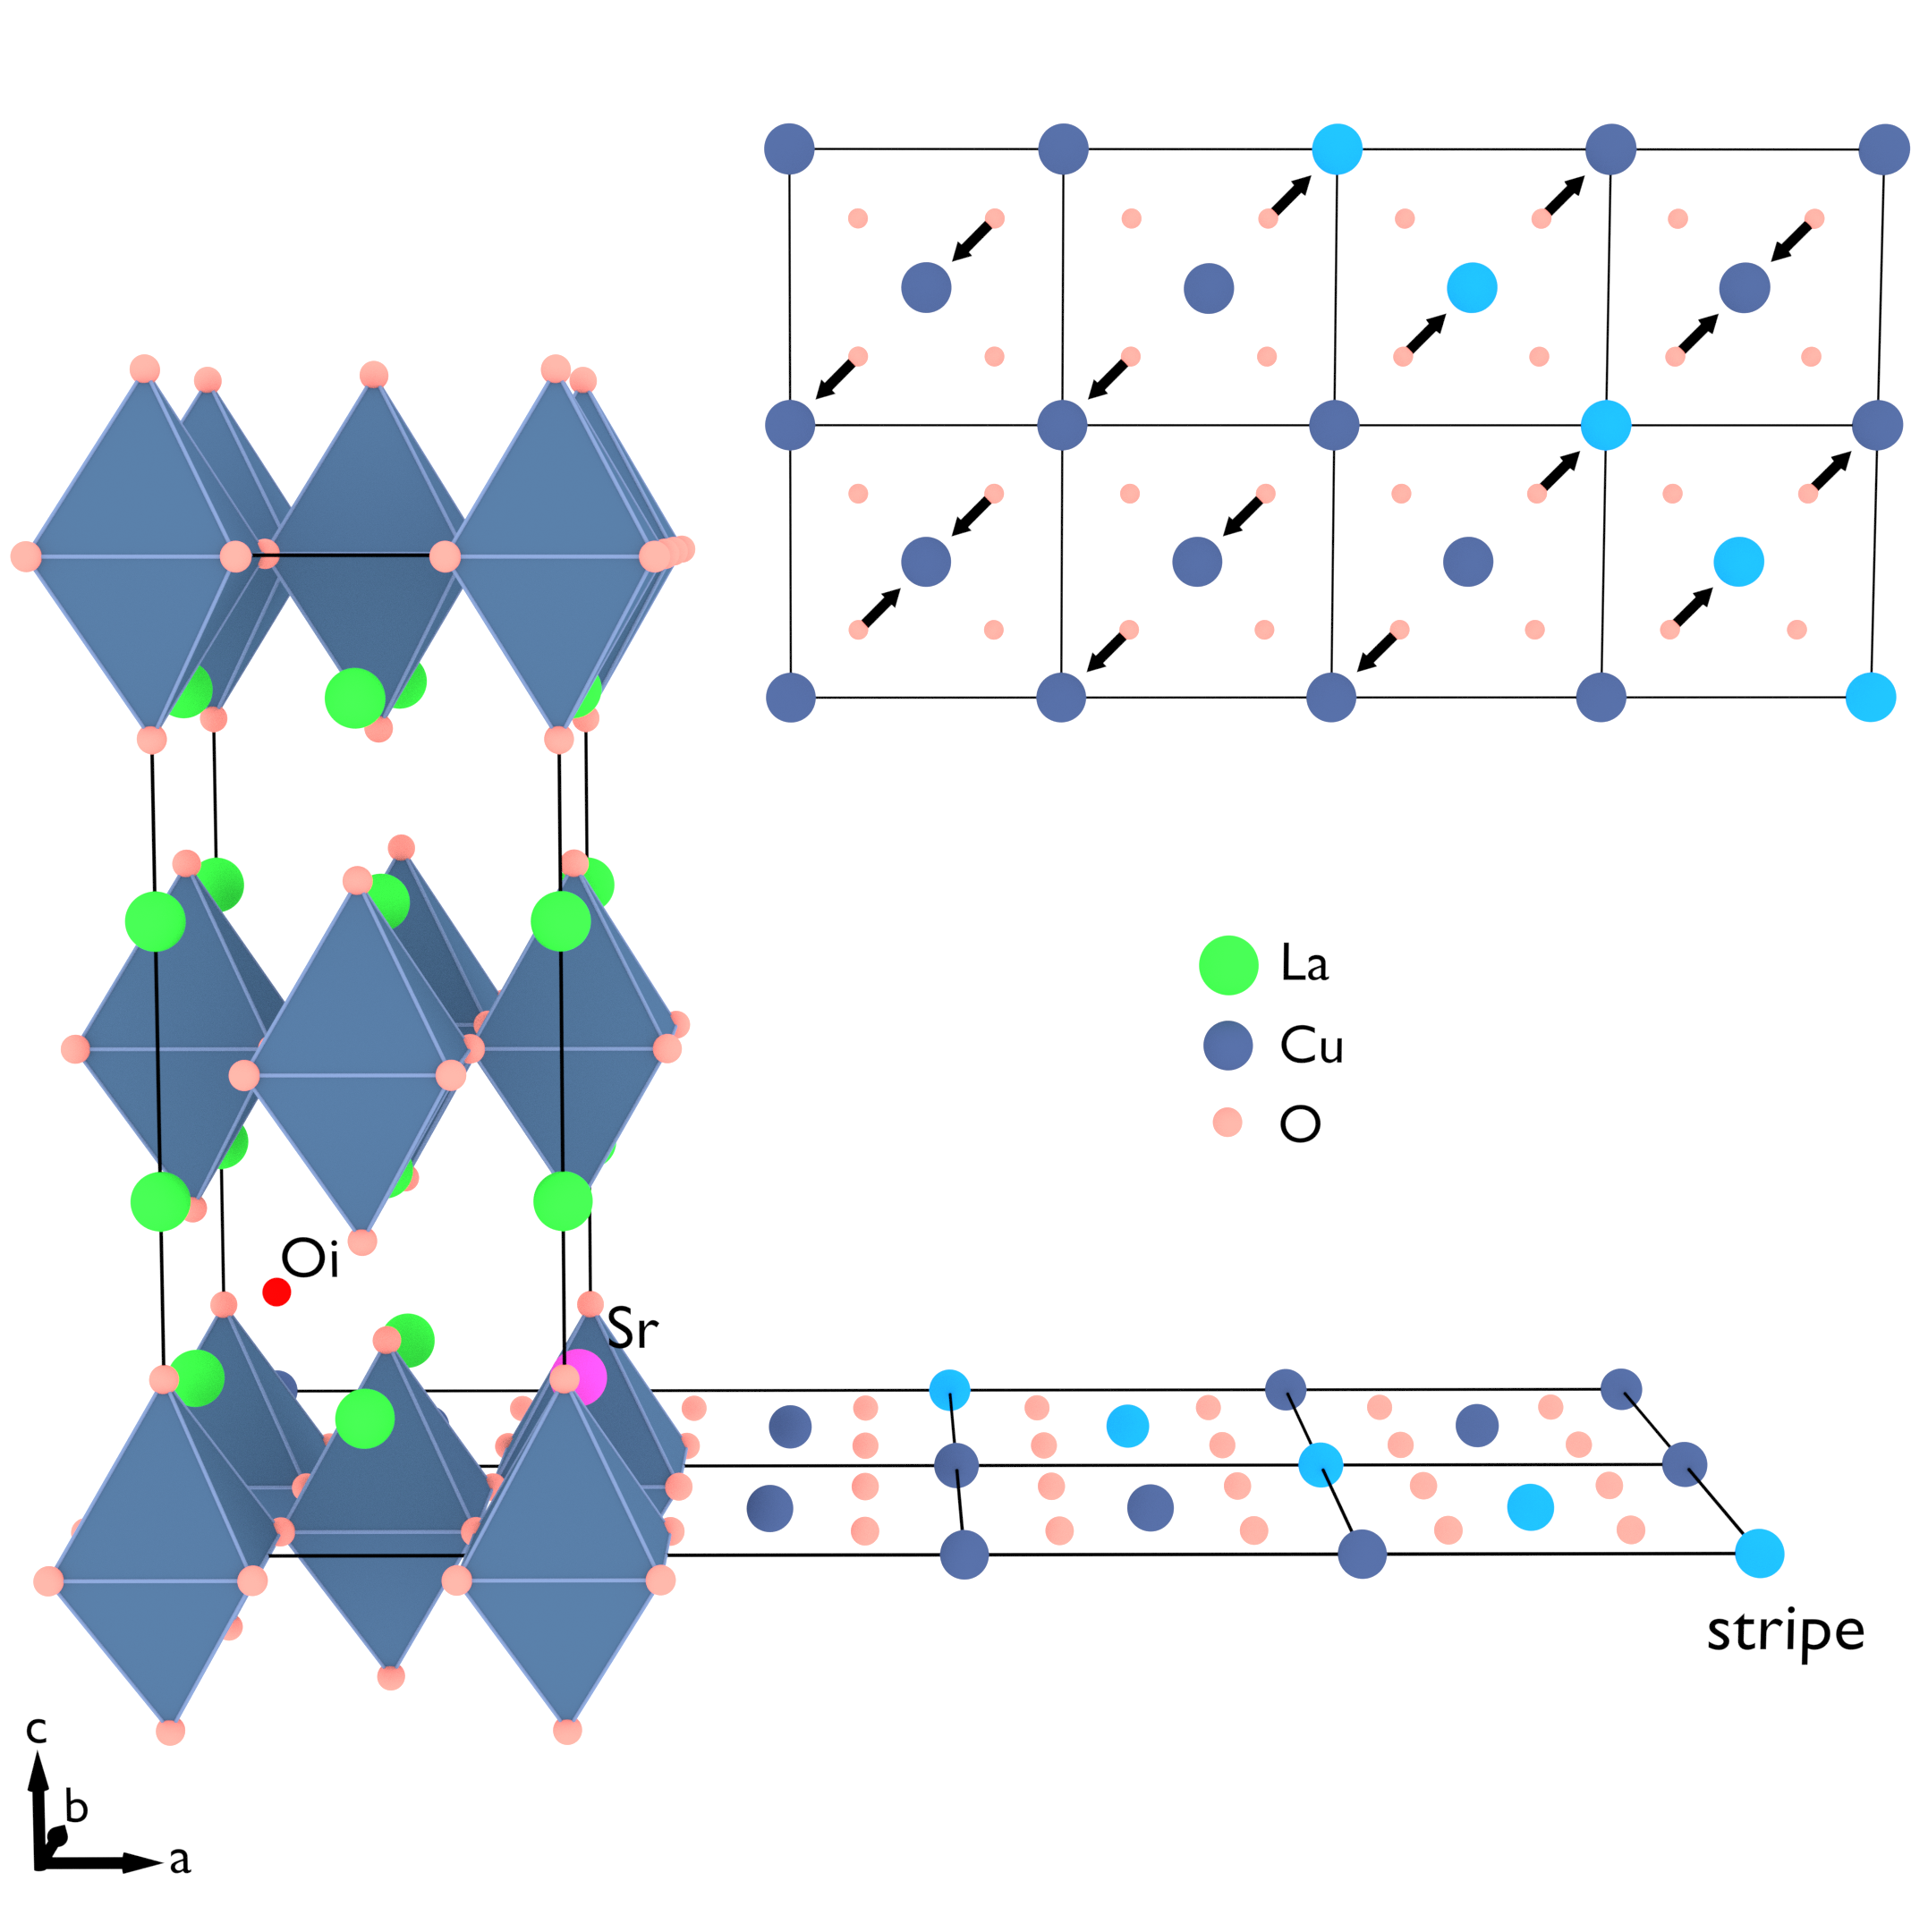
\includegraphics[width=0.7\textwidth]{fig/anomaly/overview.png}
    \caption[Crystal structure annotated with phonon at (0.25,0.25,0) and stripe order]{Sketch of crystal LSCO+O crystal structure containing two distinct dopants in a $4 \times 2 \times 1$ orthorhombic unit cell. The two singular Sr/O dopants correspond to a hole doping of $n_h = \frac{3}{32} \approx 0.09$. Dark blue are magnetic Cu sites while light blue represents hole-rich Cu sites. This period-4/8 segregation into charge/magnetic regions is known as stripe formation \cite{Tranquada1995}. Inset: Possible matching of stripe dynamics with the Cu-O bond stretching mode at q=$(0.25,0.25,0)$ as proposed by \citeauthor{Kaneshita2002} \cite{Kaneshita2002}.}
    \label{fig:crystal_anomaly}
\end{figure}

\begin{figure}
    \centering
    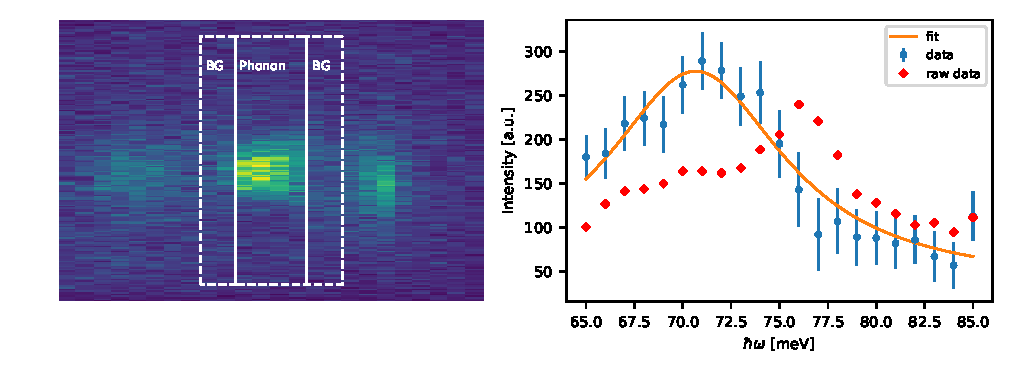
\includegraphics[width=0.54\textwidth]{fig/anomaly/data_reduction.pdf}
    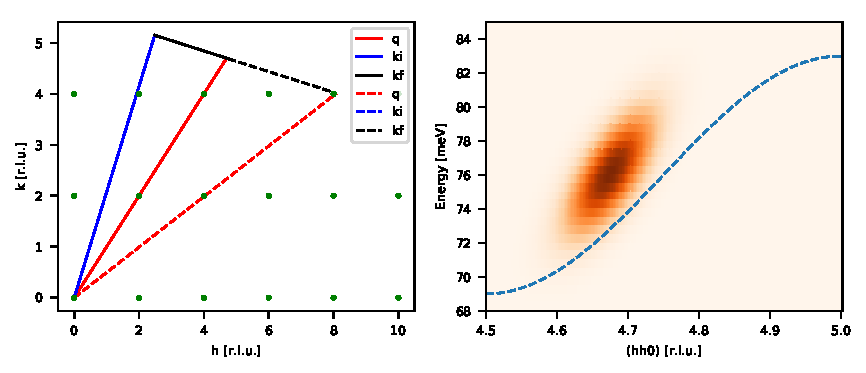
\includegraphics[width=0.45\textwidth]{fig/anomaly/spurion.pdf}
    \caption[IMPS data reduction and Spurion vizualisation]{\textbf{Top-left:} Raw data (summed from one constant-$Q$ scan) from the IMPS 2D detector. The phonon signal is observed in the central area and spurious signal is seen towards the edges. Broken white lines mark the areas used for data reduction. \textbf{Bottom-left:} Result of data reduction using the defined areas. We are clearly able to separate the phonon and spurious signal with this procedure. \textbf{Top-Right:} Scattering triangle responsible for the A-type spurious scattering (broken lines) at $Q=(4.7,4.7,0)$. The culprit is the (8,4,0) reflection. \textbf{Bottom-right:} Simulated effect of the (8,4,0) reflection on a $Q$-$\hbar\omega$ map assuming a Gaussian spurious signal depending on distances in $Q$. Broken line represents a `normal' (not anomalous) dispersion in this region.}
    \label{fig:imps_data_reduction}
\end{figure}

\begin{figure}
    \centering
    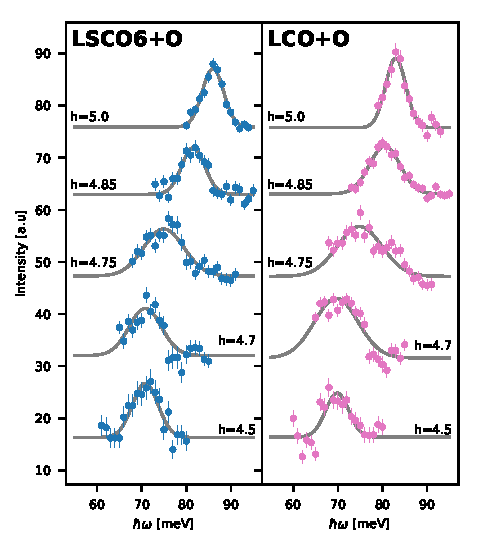
\includegraphics[width=0.49\textwidth]{fig/anomaly/selected.pdf}
    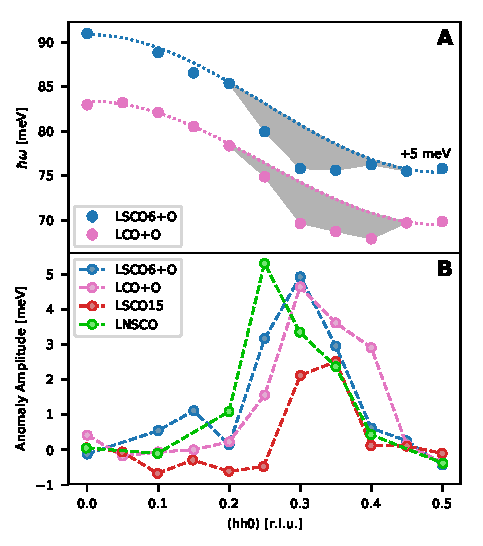
\includegraphics[width=0.49\textwidth]{fig/anomaly/disp_aa_2.pdf}
    \caption[Phonon anomaly data and dispersion]{\textbf{Left:} Raw data for LSCO6+O and LCO+O obtained with IMPS detector at IN8, ILL. Fits to Gaussian lineshape. \textbf{Right:} (A) Dispersion of LSCO6+O and LCO+O obtained from peak positions of the raw data. (B) Comparison of the anoamly amplitude (shaded gray area) between LSCO6+O, LCO+O, LSCO15 ($T_\text{c} \approx \SI{40}{\kelvin}$) and LNSCO ($x=0.12$, insulating).}
    \label{fig:anomaly_rawdata}
\end{figure}

\begin{figure}
    \centering
    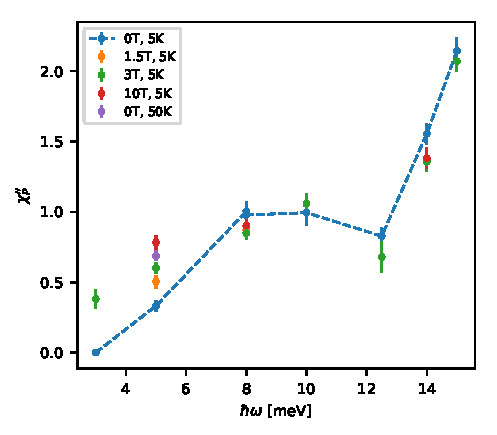
\includegraphics[width=0.49\textwidth]{fig/anomaly/chi.pdf}
    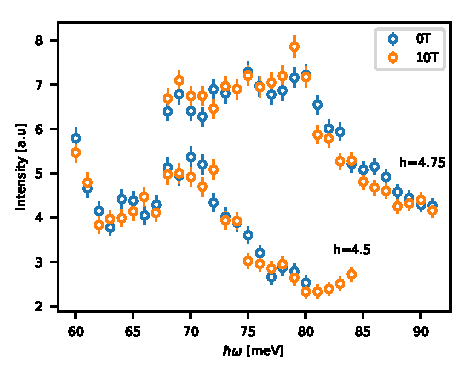
\includegraphics[width=0.49\textwidth]{fig/anomaly/field_selected.pdf}
    \caption[LSCO6+O magnetic field effect on fluctuations and phonon]{\textbf{Left:} Imaginary part of the magnetic susceptibility in LSCO6+O as a function of energy transfer, field and temperature. As shown, a field of \SI{3}{\tesla} is sufficient to open a gap in the magnetic excitation spectrum. \textbf{Right:} Raw phonon data at anomalous ($h=4.75$) and normal $h=4.5$ wave vectors as a function of field. Contrary to the magnetic excitation spectrum, the anomalous phonon does not appear to be modified by an applied field.}
    \label{fig:phonon_chi_field}
\end{figure}

\section{Things deleted from paper}

\subsection{PDW Stuff in detail}
As is usual with the cuprates, it is difficult to find a framework that captures all of the experimental evidence. With that in mind, we relate our findings to the concept of intertwined orders, while keeping in mind that oxygen-doped samples are macroscopically phase seperated. Intertwined orders are described with reference to pair-density-wave (PDW) superconductivity as the parent microscopic order from which $d$-wave superconductivity, magnetic order, charge order and others emerge\cite{Fradkin2015}. The PDW formalism predicts simultaneous ordering temperatures, gapless magnetic excitations\cite{Christensen2016} and an `electronic liquid crystal' phase\cite{Kivelson1998} that emerges from transverse fluctuations in the charge-density-waves (CDW) of neighbouring stripes. These fluctuations then become the fundamental degrees of freedom relevant to superconductivity. This is consistent with the fact that we see the phonon anomaly whenever the CDW is present, regardless of the nature of the transverse fluctuations. This could potentially explain the `sharper' phonon anomaly in static stripe-ordered LNSCO (Figure DISPERSION)\todo{Note that I have never seen Reznik or Tranquada imply this connection, so it might be a bit too speculative?}.

Returning to LCO+O, LSCO6+O and LSCO15, this would explain the discrepancy in magnetic signatures while still having similar $T_\text{c}$ and phonon anomaly, if we assume that the magnetic domains between the fluctuating stripes can be tuned separately\todo{not sure if this is the case, but in the original papers, electronic liquid phase is described without considering magnetism}. In the case of static charge order and magnetism, this is not the case\cite{Christensen2014}. Another scenario is one in as sample without separate domains of static and fluctuating stripes in which the magnetic field only modifies spectral weight at low energies while not affecting the phonon mode at $\approx 80\,\text{meV}$. A measurement of the phonon anomaly in field of static stripe ordered LSCO ($x=0.12$) would help resolve these issues. A significant disceprency in this interpretation is that fact that LSCO+O is macroscopically phase separated, so the question remains if the two phases are entirely segregated or if exactly one of them contains the physics described here\todo{Linda can you weigh in?}.

\subsection{Chemical disorder - not sure if relevant}
It has been suggested that the inhomogeneous charge distribution due to dopant ions can cause a renormalization of elementary excitations\cite{Park2011}. By adding optimally superconducting, oxygen-doped samples to the list of samples with strong phonon anomalies, we rule out any connection between the phonon anomaly and specific dopant disorder.

\subsection{Discussion}
The results of our measurements (Figure DISPERSION) clearly show the similarity of anomalous behavior between optimally doped LSCO15 and oxygen-overstoichiometric L(S)CO+O. Due to the difference in dopant species, we believe that an immediate result of these measurements is a confirmation of the relationship between fluctuating charge order in the CuO$_2$ planes and the giant phonon anomaly as proposed by \citeauthor{Reznik2012}\cite{Reznik2012}. In the following discussion, we work under the hypothesis that fluctuating charge order in LSCO15 and L(S)CO+O is expressed in the same way despite the different chemistries and bulk characteristics of the two compounds. We start by reviewing some important results from LSCO literature.

It is well established that stripe order is ubiquitous in the cuprates, but a correlation with superconductivity remains elusive and maintaining an internal consistency between measurements is challenging. Neutron scattering, $\mu$SR, NQR and NMR experiments of $T_m$ have shown that static magnetic stripes in LSCO appear at $x=0.03$, take a maximum at $x=0.125$ (where $T_\text{c} \approx 25$ has a minimum) before disappearing abruptly\cite{Julien2003, Hirota2001}. In contrast dynamic magnetic stripes have been observed throughout the superconducting dome, with a gap opening in the spin excitation spectrum for $0.125 < x < 0.20$\cite{Kofu2009, Lee2000, Gilardi2004}. On the other hand, samples considered in this letter both exhibit static magnetic stripes\todo{REF?}, have a gap of 3 meV (LSCO+O)\todo{REF?} and no gap (LCO+O)\cite{Wells1997, Jacobsen2018}, while sharing an optimal $T_\text{c} \approx 40\,\text{K}$. With these results in mind, it is natural to question a trivial relationship between static and dynamic magnetic stripes. Recent measurements by \citeauthor{Jacobsen2018} on LCO+O show a discrepancy in the momentum-transfer of static and dynamic magnetic stripes\cite{Jacobsen2018}, directly showing that the perceived connection might be coincidental.

If the magnetic signal from stripes occur with a modulation of $\delta_\text{m}$, the charge component appears with a modulation of $\delta_\text{c} = 2\delta_\text{m}$. In LSCO static charge stripes have been found for a narrow range of doping ($0.12 < x < 0.13$)\cite{Thampy2014, Croft2014} at the expected position with $\delta_\text{c} = 0.25$. In addition, the static magnetic and static charge stripes have an identical response to magnetic field in LSCO ($x=0.12$) below $T_\text{c}$, indicating a strong connection between the two phenomena\cite{Christensen2014}. Dynamic charge order has, to our knowledge, never been directly observed in LSCO.

Despite the experimental inconsistencies outlined above, we believe that unifying observations of stripe order would be a significant step in our quest to understand superconductivity in the cuprates. The nature of dynamic charge order is a significant missing piece in the stripe picture. The `giant' phonon anomaly observed in LBCO, LSCO, YBCO and now L(S)CO+O represents significant progress in finding said piece. While phonon anomalies, in general, can happen for a number of reasons, the connection to stripe order comes in multiple flavours\cite{Reznik2012}. First, the phonon anomaly obeys the symmetry of charge stripes appearing at $\delta_\text{c} \approx 0.25$. The 1D nature of the phonon anomaly is verified from experiments showing a disappearance of the phonon anomaly by deviating slightly from the Cu-O bond direction\todo{REF?}. ARPES and Inelastic X-ray Scattering (IXS) experiments on LSCO ($x=0.20$)\cite{Park2014} have shown that the phonon anomaly cannot be caused by Fermi Surface nesting (Kohn anomaly). Theoretically, it has been proposed that the phonon anomaly can be explained as steeply dispersing charge fluctuations intersecting the optical phonon branch\cite{Kaneshita2002}

Perhaps the most appealing feature of the phonon anomaly is the apparent correlation with $T_\text{c}$. In LSCO ($x=0.20$ and $x=0.15$), the anomaly amplitude is larger than for samples outside or on the edge of the superconducting dome. The samples studied in this letter follow this trend by having slightly larger $T_\text{c}$ and anomaly amplitudes compared to their LSCO15 cousin.

With this in mind, we believe that the results contained in Figure \ref{fig:dispersion} proves the hypothesis of \citeauthor{Reznik2012} \cite{Reznik2012} that the phonon anomaly is connected to charge fluctuations in the CuO$_2$-planes. Our samples are chemically distinct to LSCO15 and each other, but exhibit identical behavior in terms of the energy scale of the phonon dispersion and the anomaly amplitude. The lack of field effect in Figure FIELD is surprising, but consistent with results on YBCO\todo{REF?}. On the other hand, the phonon anomaly has almost no temperature dependance, indicating that the fluctuations are extremely robust.

\subsection{Old stuff 1}
In addition, the magnitude of this gap $E_g$ has been suspected to track $T_\text{c}$ through the relation $T_c = 1.5 E_\text{g}/k_\text{B}$\cite{Kofu2009}. The samples considered in this letter contradicts this suspicion by having comparable $T_\text{c} \approx 40\,\text{K}$, while LCO+O exhibits no gap\cite{Jacobsen2018,Wells1997} while LSCO+O has a gap of $E_g \approx 3.5$ meV, similar to LSCO15\cite{Lee2000}.


The controversy is rooted in the fact that static stripe order appears to suppress superconductivity while their fluctuations have been proposed to promote superconductivity. It thus becomes natural to ask if the static and dynamic stripe order arises from the same electronic phenomenon and if they are separate phases that can be tuned individually. 

In either case, stripe order has manifestations of competing orders. A notorious example is the `$T_\text{c}$ anomaly' in LSCO, where a suppression of $T_c$ happens at $n_h=\frac{1}{8}$ along with measurable static magnetic and charge order\cite{Christensen2014,Croft2014,Thampy2014}, which is not present in optimally doped LSCO15. In non-superconducting, tetragonal LNSCO and LBCO, similar features have been observed\cite{Wilkins2011}. In addition, \citeauthor{Christensen2014} have shown, by performing experiments in magnetic fields, that the static charge and spin order is connected\cite{Christensen2014}.

Fluctuating magnetic order has been extensively studied throughout the LSCO phase diagram, revealing a connection between 1) the incommensurate modulation $\delta$ of the antiferromagnetic parent phase and 2) the hole doping $n_h$. $\delta$ is equal to $n_h$ up to a saturation at $\delta = n_h = \frac{1}{8}$[yamada], once again stressing the ubiquity of this `$\frac{1}{8}$ phase' in the cuprates.

A playground for understanding this `zoo' of orders is the LSCO+O system, which separates\cite{Mohottala2006} into distinct magnetic ($n_h=\frac{1}{8}$) and superconducting phases\cite{Udby2013}. In addition, the mobile nature of the dopants severely reduces flux pinning\cite{Mohottala2008}, indicating that annealed disorder allows the superconducting part of the sample to emerge in a cleaner way.

From the $T_c$ anomaly in LSCO, phase separation in LSCO+O, the incommensurability $\delta$ of magnetic fluctuations and the insulating nature of LNSCO and LBCO12, we believe that the `$\frac{1}{8}$ phase' is a necessary, but not sufficient precursor for superconductivity. The question then remains: How are the magnetic and charge fluctuations related to this phase and how are they expressed in experiments?

An appealing picture that unite these features is one of simultaneous structural and electronic phase separation in real space, with 1) the $\frac{1}{8}$ non-superconducting phase  expressed by static order and 2) the superconducting phase containing fluctuating charge and magnetic order. Due to the quenched disorder of LSCO this separation only becomes apparent around $n_h = \frac{1}{8}$, while the annealed disorder in LSCO+O results in detectable phase separation at optimal doping.

While subtle, several experiments support this picture. \citeauthor{Kofu2009} reports a different origin of spin fluctuations in LSCO around the $\frac{1}{8}$ anomaly ($x=0.125,0.13.0.135$) above and below a spin gap at $\approx 4$ meV through detailed measurements of the intrinsic linewidth of the excitations. Recently \citeauthor{Jacobsen2018}\cite{Jacobsen2018} reported a different origin in momentum space of the static and dynamic spin stripes through high-resolution measurements of the incommensurability $\delta$ in LCO+O (The same sample studied in this letter). 

Real-space structural phase separation in LCO+O has been probed by X-ray micro-diffraction. \citeauthor{Poccia2012} showed a spatial anti-correlation between two kinds of oxygen orderings\cite{Poccia2012} and in the single-layered cuprate HBCOO ($T_c = 95\,\text{K}$) containing oxygen interstitials, \citeauthor{Campi2015} found a nano-scale spatial anti-correlation between Oxygen-rich and CDW-rich regions\cite{Campi2015}.

We hypothesize that novel charge fluctuations contain vital elements of the pairing mechanism in cuprates, but that SC only arises when the stripe phase is realized locally. In this picture charge fluctuations survive above $T_c$, but SC is realized only as we approach static stripe order.

Starting from our assumption that the phonon anomaly is an expression of steeply dispersing charge fluctuations intersecting an optical phonon branch\cite{Kaneshita2002}, the above picture explains the difference between LSCO15, LNSCO and L(S)CO+O. LNSCO is close to superconductivity, but the specific local structure induced by the addition of Nd$^3+$ ions prevents the `good' charge fluctuations to separate from the $\frac{1}{8}$ phase. The stronger local energetics due to structure produces a steeper dispersion, resulting in a strongly peaked anomaly at $h=\frac{1}{4}$ (charge component of $\frac{1}{8}$ phase). LSCO15 and L(S)CO+O, on the other hand, have an optimal local structure allowing superconductivity to emerge unscathed. The slightly better superconducting properties of the oxygen-overstoichiometric samples are thus reflected in the broader and stronger anomalies. This is also consistent with the experiments performed by \citeauthor{Park2014}\cite{Park2014}, where the strength of the anomaly is found to scale with $T_c$.

Finally, even though we are able to populate the $\frac{1}{8}$ phase with a magnetic field in LSCO+O (Udby et al, to be published) the charge fluctuations connected to SC are completely untouched by a field of 10T ($\ll H_{c2}$) and this is reflected in the absence of modifications of the anomaly (See Figure FIELD).
